\documentclass[10pt,a4paper]{article}
\usepackage[T1]{fontenc}
\usepackage[utf8]{inputenc}
\usepackage{graphicx}
\usepackage{caption}
\usepackage{subcaption}
\usepackage{tabularx}
\usepackage{helvet}
\usepackage{hhline}
\usepackage{verbatim}
\usepackage{keystroke}
\usepackage{hyperref}
\usepackage[a4paper,margin=1in]{geometry}
\usepackage[polish]{babel}
\usepackage{float}

\renewcommand\familydefault{\sfdefault}

\begin{document}
\begin{titlepage}
	\centering
	{\Large Wydział Matematyki i Nauk Informacyjnych Politechniki Warszawskiej \par}
	\vspace{1cm}
	
\includegraphics[width=0.2\textwidth]{logo.png} \par
	\vspace{5cm}
	{\LARGE Chess3D -- wizualizacja gry w szachy \par}
	\vspace{0.5cm}
	{\Large Bartłomiej Dach \par}
	\vspace{1.5cm}
	{\Large Wersja 1.3 \par}
	\vspace{1.5cm}
	{\Large \today \par}
\end{titlepage}
Lista zmian w dokumencie:
\begin{table}[H]
\def\arraystretch{1.5}
\begin{tabularx}{\textwidth}{|l|l|X|l|}
	\hline
	\textbf{Data} & \textbf{Autor} & \textbf{Opis zmian} & \textbf{Wersja} \\
	\hline
	14.12.2016 & Bartłomiej Dach & Dodanie specyfikacji wymagań & 1.0 \\
	\hline
	15.12.2016 & Bartłomiej Dach & Rozszerzenie opisu biznesowego, dodanie szkicu architektury & 1.1 \\
	\hline
	15.01.2017 & Bartłomiej Dach & Dodanie wymagań, instrukcji instalacji oraz obsługi aplikacji & 1.2 \\
	\hline
	17.01.2017 & Bartłomiej Dach & Dodanie scenariuszów i wyników testów akceptacyjnych, uszczegółowienie architektury & 1.3 \\
	\hline
\end{tabularx}
\end{table}

\tableofcontents
\newpage

\section{Specyfikacja}

\subsection{Opis biznesowy}
Celem aplikacji \emph{Chess3D} jest wyświetlanie trójwymiarowej wizualizacji. Przedstawia ona scenę składającą się z szachownicy oraz pionków szachowych, oświetlanych światłem stożkowym.

Użytkownik aplikacji może zaznaczyć dowolny pionek na planszy, a następnie wskazywać pole, na który dany pionek powinien być przesunięty. Ruchy wykonane przez użytkownika nie muszą być prawidłowymi ruchami szachowymi, tj. ich poprawność pod tym kątem nie jest sprawdzana przez aplikację. Po wyspecyfikowaniu ruchu aplikacja w czasie rzeczywistym wyświetla animację przesunięcia pionka w nowe miejsce.

W zakresie projektu znajduje się również demonstracja kilku klasycznych metod symulacji światła dla obiektów trójwymiarowych, a mianowicie:
\begin{itemize}
	\item modele oświetlenia sceny:
	\begin{itemize}
		\item model Phonga \cite{phong75},
		\item model Blinna-Phonga \cite{blinn77},
	\end{itemize}
	\item tryby cieniowania trójkątów:
	\begin{itemize}
		\item cieniowanie płaskie,
		\item cieniowanie Gouraud \cite{gouraud71},
		\item cieniowanie Phonga \cite{phong75}.
	\end{itemize}
\end{itemize}
Użytkownik powinien mieć możliwość wyboru powyższych metod, skutkujący natychmiastową aktualizacją wyglądu sceny.

Dodatkowo, do wyboru przez użytkownika powinny być następujące trzy kamery, zmieniające perspektywę postrzegania sceny:
\begin{itemize}
	\item kamera nieruchoma, obejmująca całość szachownicy; usytuowanie tej kamery powinno umożliwiać łatwe wykonanie ruchu, czyli wybranie przez użytkownika pionka i pola,
	\item kamera nieruchoma, śledząca ruch ostatnio przesuniętego pionka,
	\item kamera ruchoma, związana z ostatnim poruszanym pionkiem na szachownicy.
\end{itemize}

Renderowanie sceny powinno odbywać się w trybie \emph{software}, tzn. obliczenia związane z wyświetlaniem obrazu mają używać procesora, zamiast jednostek \hyperref[abbr:gpu]{GPU}. Potok renderowania powinien być zaimplementowany od podstaw oraz wzorować się na istniejącym popularnym schemacie używanym w wielu bibliotekach graficznych 3D, takich, jak m.in. OpenGL, składającym się z następujących kroków:
\begin{itemize}
	\item transformacja współrzędnych (współrzędne świata, kamery),
	\item rzut na płaszczyznę,
	\item obcinanie wielokątów oraz porządkowanie ich względem odległości od kamery,
	\item wypełnianie wielokątów zgodnie z przyjętym modelem oświetlenia.
\end{itemize}

\newpage

\subsection{Wymagania biznesowe}

\subsubsection*{Przypadki użycia}

Przypadki użycia aplikacji przedstawione są na poniższym diagramie UML.

\begin{figure}[H]
	\centering
	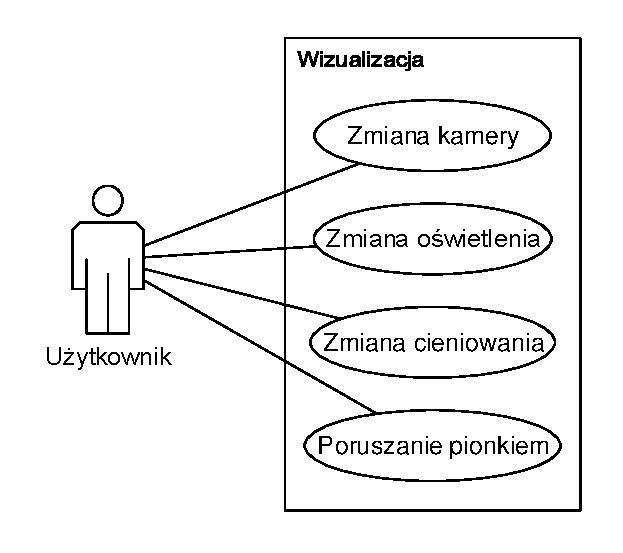
\includegraphics[width=7cm]{use-case.pdf}
	\caption{Diagram przypadków użycia}
\end{figure}

\begin{table}[H]
	\begin{tabularx}{\textwidth}{|l|X|X|}
		\hline
		\textbf{Nazwa} & \textbf{Opis} & \textbf{Odpowiedź systemu} \\
		\hline
		Zmiana kamery &
		Zmiana kamery w wizualizacji na jedną z trzech poniższych opcji:
		& Aktualizacja wizualizacji uwzględniająca wybór kamery.
		\\
		& $\bullet$ kamera nieruchoma, z widokiem na całą scenę, & \\
		& $\bullet$ kamera nieruchoma, śledząca ostatnio poruszony pionek, & \\
		& $\bullet$ kamera ruchoma, związana z ostatnio poruszonym pionkiem. & \\
		\hline
		Zmiana oświetlenia &
		Zmiana modelu oświetlenia sceny na model Phonga lub model Blinna. &
		Aktualizacja wizualizacji uwzględniająca wybrany model oświetlenia. \\
		\hline
		Zmiana cieniowania &
		Zmiana trybu cieniowania sceny na jeden z poniższych: &
		Aktualizacja wizualizacji uwzględniająca wybrany tryb cieniowania. \\
		& $\bullet$ cieniowanie stałe, & \\
		& $\bullet$ cieniowanie Gouraud, & \\
		& $\bullet$ cieniowanie Phonga. & \\
		\hline
		Poruszanie pionkiem &
		Przesunięcie pionka na nowe pole po wybraniu pionka i pola. &
		Animacja poruszania się pionka, wyświetlana w czasie rzeczywistym. \\
		\hline
	\end{tabularx}
	\caption{Opisy przypadków użycia}
\end{table}

\newpage

\subsection{Wymagania niefunkcjonalne}

W trakcie analizy rozpoznane zostały następujące wymagania niefunkcjonalne:

\begin{table}[H]
	\begin{tabularx}{\textwidth}{|l|X|}
		\hline
		\textbf{Obszar wymagań} & \textbf{Opis} \\
		\hline
		Użyteczność & Aplikacja powinna posiadać dwa tryby działania: okienkowy oraz pełnego ekranu. \\
		\hline
		Niezawodność & Na obrazie generowanym przez aplikację nie powinny być widoczne żadne artefakty lub zniekształcenia spowodowane błędami renderingu. \\
		\hline
		Wydajność & Aplikacja powinna być w stanie generować kolejne klatki obrazu w czasie krótszym niż 1 sekunda (płynność większa niż 1 klatka na sekundę). \\
		\cline{2-2}
		& Aplikacja powinna zajmować mniej niż 500 MB pamięci RAM systemu. \\
		\hline
		Utrzymanie & Wraz z aplikacją zostanie dołączona instrukcja obsługi. \\
		\cline{2-2}
		& Aplikacja będzie wspierała wczytywanie modeli pionków szachowych z plików \texttt{.obj} lub innych wspieranych przez narzędzia do modelowania 3D. \\
		\hline
	\end{tabularx}
	\caption{Lista wymagań niefunkcjonalnych dla aplikacji}
\end{table}

\subsection{Harmonogram projektu}

Harmonogram zadań przedstawiony jest na poniższym diagramie Gantta:

\begin{figure}[H]
	\centering
	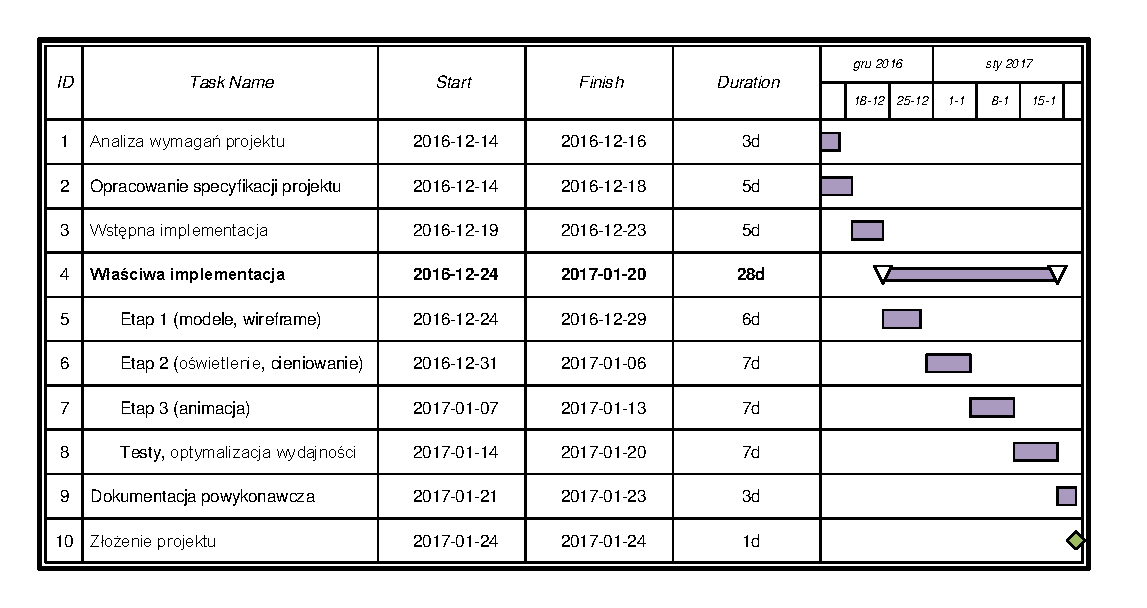
\includegraphics[width=14cm]{gantt-chart.pdf}
	\caption{Diagram Gantta przedstawiający planowany harmonogram prac}
\end{figure}
Poniżej przedstawione zostały kamienie milowe wchodzące w skład realizacji projektu.
\begin{enumerate}
	\item 16 grudnia 2016 -- zakończenie analizy wymagań projektu,
	\item 18 grudnia 2016 -- uzgodnienie specyfikacji projektu,
	\item 23 grudnia 2016 -- zakończenie wstępnej implementacji,
	\item 20 stycznia 2017 -- zakończenie właściwej implementacji,
	\item 23 stycznia 2017 -- zakończenie prac nad dokumentacją powykonawczą,
	\item 24 stycznia 2017 -- złożenie projektu wraz z pełną dokumentacją.
\end{enumerate}

\newpage

\subsection{Architektura rozwiązania}

Ze względu na spełniane funkcjonalności aplikacja została podzielona na komponenty w sposób zaprezentowany na poniższym diagramie:

\begin{figure}[H]
	\centering
	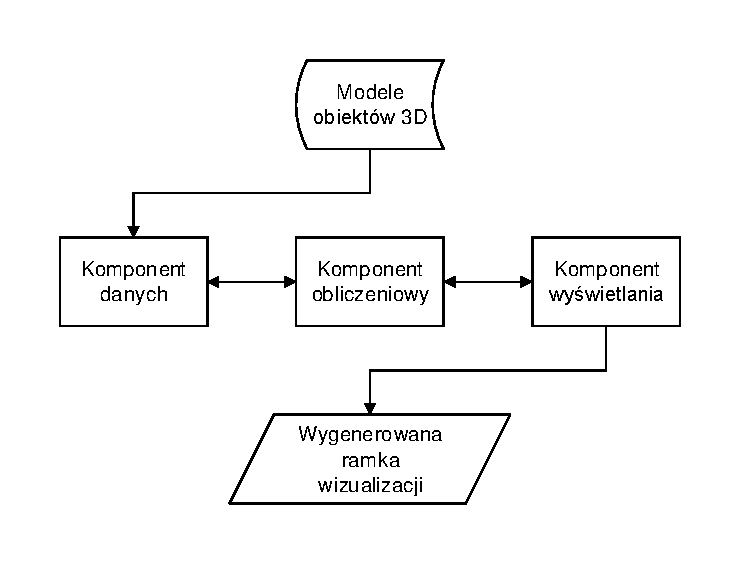
\includegraphics[width=10cm]{component-chart.pdf}
	\caption{Diagram komponentów aplikacji}
\end{figure}

\paragraph{Komponent danych}
Odpowiada za wczytanie z dysku danych związanych ze sceną, takich, jak: dane modeli wykorzystanych w scenie, położenie i parametry oświetlenia obiektów. Zawiera on również klasy reprezentujące te obiekty, których używa komponent obliczeniowy. Proces wczytywania modeli jest wspomagany przez bibliotekę \emph{Assimp} \cite{assimp}.

\paragraph{Komponent obliczeniowy}
Jego rolą jest przetworzenie wczytanych z plików wejściowych danych i dokonanie właściwych obliczeń związanych z wizualizacją, tj. zmianę układów współrzędnych, rzutu na płaszczyznę oraz symulację oświetlenia. Do wykonywania obliczeń wykorzystana zotała biblioteka \emph{Eigen} \cite{eigen}.

\paragraph{Komponent wyświetlania}
Wykorzystuje obliczenia wykonane przez powyższy komponent do właściwego tworzenia obrazu dwuwymiarowego i wyświetla go na ekranie. Ponadto obsługuje polecenia użytkownika, wydawane za pośrednictwem interfejsu graficznego, i przekazuje informacje o nich do pozostałych komponentów. W tym komponencie wykorzystane zostały funkcjonalności biblioteki \emph{Simple DirectMedia Layer 2.0} \cite{sdl}.

W celu uzyskania jak największej wydajności, aplikacja stworzona została w języku C++.

\begin{figure}[H]
	\centering
	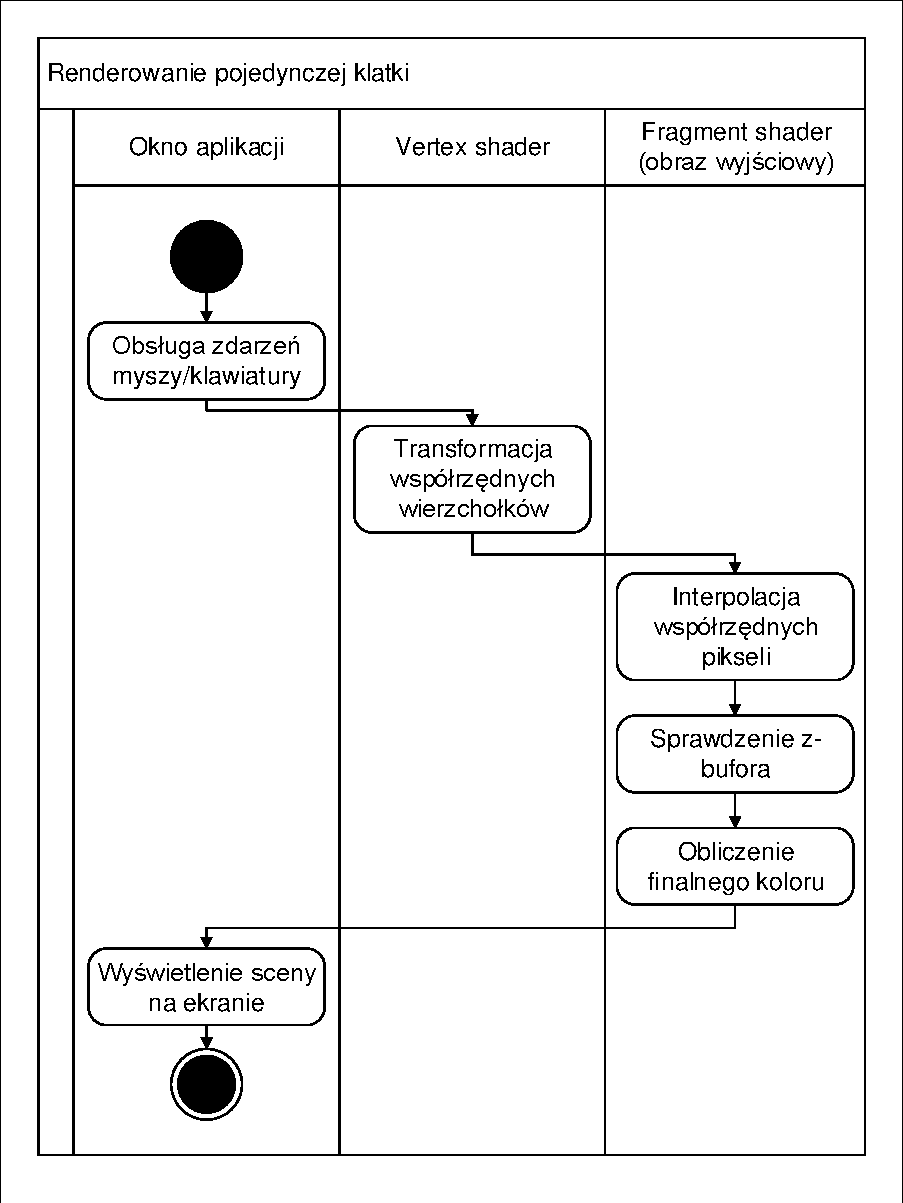
\includegraphics[width=10cm]{frame-render-activity.pdf}
	\caption{Diagram aktywności ukazujący przebieg renderowania pojedynczej klatki}
\end{figure}

Główna pętla aplikacji składa się z następujących elementów:
\begin{itemize}
	\item obsługa nadchodzących zdarzeń myszy i klawiatury,
	\item jeśli jest to potrzebne, odrysowanie sceny.
\end{itemize}
Na rysowanie sceny składają się następujące kroki:
\begin{enumerate}
	\item użycie \emph{vertex shadera} w celu transformacji współrzędnych w układzie świata do współrzędnych w układzie kamery,
	\item użycie wybranego przez użytkownika \emph{fragment shadera} w celu zapisania kolorów kolejnych pikseli do bufora. Dla każdego piksela trójkątów poszczególnych modeli wykonywane są następujące kroki:
	\begin{itemize}
		\item interpolacja współrzędnych w układzie kamery na podstawie współrzędnych piksela na ekranie,
		\item sprawdzenie (i ewentualnie nadpisanie) z-bufora,
		\item jeśli bufor został nadpisany, wybrany model oświetlenia jest użyty do obliczenia finalnego koloru danego piksela. 
	\end{itemize}
	\item jeżeli nie trwa animacja, używany jest dodatkowo specjalny \emph{fragment shader}, aby wyliczyć tzw. \emph{click mapę}. Jest to tekstura (bufor w pamięci), który dla każdego piksela ekranu zapisuje indeks obiektu, który zajmuje ten piksel i jest najbliżej ekranu. W ten sposób sprawdzenie, jaki pionek i pole zostały trafione, sprowadza się do wczytania wartości z odpowiedniego miejsca tego bufora. 
\end{enumerate}

Obsługa zdarzeń związanych z myszą odbywa się za pomocą prostej maszyny stanów, przedstawionej na poniższym diagramie.
\begin{figure}[H]
	\centering
	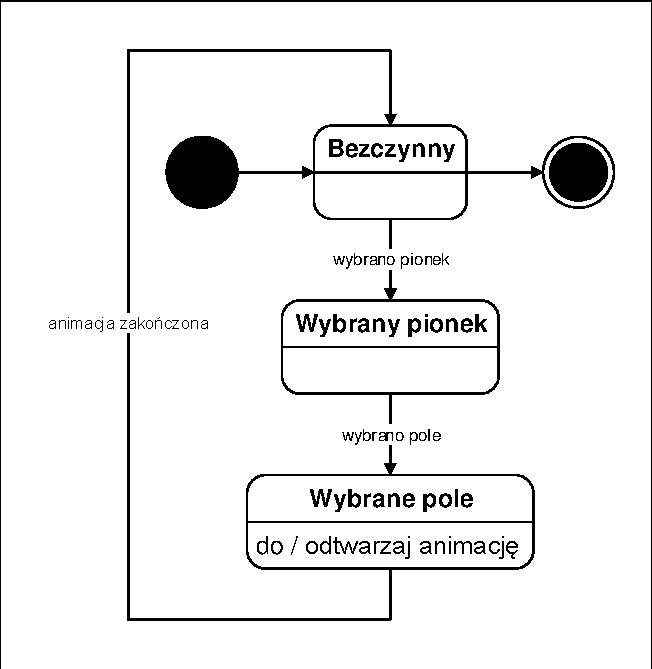
\includegraphics[width=7cm]{window-state.pdf}
	\caption{Diagram stanów -- obsługa zdarzeń myszy przez aplikację}
\end{figure}
W momencie wybrania pionka w stanie ,,Wybrany pionek'', wyświetlana jest wiadomość o błędzie.

\newpage

\section{Dokumentacja końcowa (powykonawcza)}

\subsection{Wymagania systemowe}

Do funkcjonowania programu wymagany jest system Microsoft Windows Vista lub nowszy, działający w architekturze 64-bitowej.

\subsection{Biblioteki wraz z określeniem licencji}

Poniższa tabela przedstawia listę użytych w projekcie bibliotek:

\begin{table}[H]
	\begin{tabularx}{\textwidth}{|r|l|X|l|c|}
		\hline
		\textbf{Nr} & \textbf{Komponent, wersja} & \textbf{Opis} & \textbf{Licencja} & \\
		\hline
		1 &
		Assimp 3.0.0 &
		Używana do importowania modeli zapisanych w wielu formatach używanych przez popularne narzędzia CAD/CAM. &
		\mbox{\hyperref[abbr:bsd]{BSD}} 3-Clause &
		\cite{assimp} \\
		\hline
		2 &
		Eigen 3.2.9 &
		Biblioteka do obliczeń algebry liniowej; wspiera operacje na wektorach oraz macierzach. &
		\mbox{\hyperref[abbr:mpl]{MPL}} 2.0 &
		\cite{eigen} \\
		\hline
		3 &
		FreeType 2.6.2.1 &
		Wspiera ładowanie i wyświetlanie na ekranie czcionek w formacie TrueType (\texttt{.ttf}). &
		FreeType License &
		\cite{freetype} \\
		\hline
		4 &
		SDL 2.0.5 &
		Wieloplatformowa biblioteka umożliwiająca niskopoziomowy dostęp do myszy, klawiatury oraz wyświetlanie obrazu 2D na ekranie. &
		zlib license &
		\cite{sdl} \\
		\hline
		5 &
		SDL\_ttf 2.0.14 &
		Biblioteka integrująca FreeType oraz SDL. &
		zlib license &
		\cite{sdl_ttf} \\
		\hline
	\end{tabularx}
\end{table}

\subsection{Instrukcja instalacji}

W celu zainstalowania aplikacji na dysku twardym, należy uruchomić dołączony ze źródłami projektu plik wykonywalny \texttt{installer.exe}, a następnie postępować zgodnie z instrukcjami wyświetlonymi na ekranie.

\subsection{Instrukcja uruchomienia}

Po zakończeniu instalacji należy uruchomić plik wykonywalny \texttt{Chess3D.exe}, znajdujący się w katalogu instalacji programu.

\subsection{Instrukcja użycia}

Aplikacja Chess3D składa się z pojedynczego okna, na którym wyświetlana jest wizualizacja z pionkami oraz szachownicą.

\paragraph{Wykonywanie ruchów}
Aby wykonać ruch jednym z pionków, należy kliknąć na dowolny z nich, a następnie kliknąć na żądane pole. Wówczas rozpocznie się animacja przesuwania się pionka na swoje miejsce. Nie można ruszać wielu pionków jednocześnie; należy odczekać, aż animacja się zakończy przed dokonaniem kolejnego ruchu.

\begin{figure}[H]
	\centering
	\begin{subfigure}[b]{0.45\textwidth}
		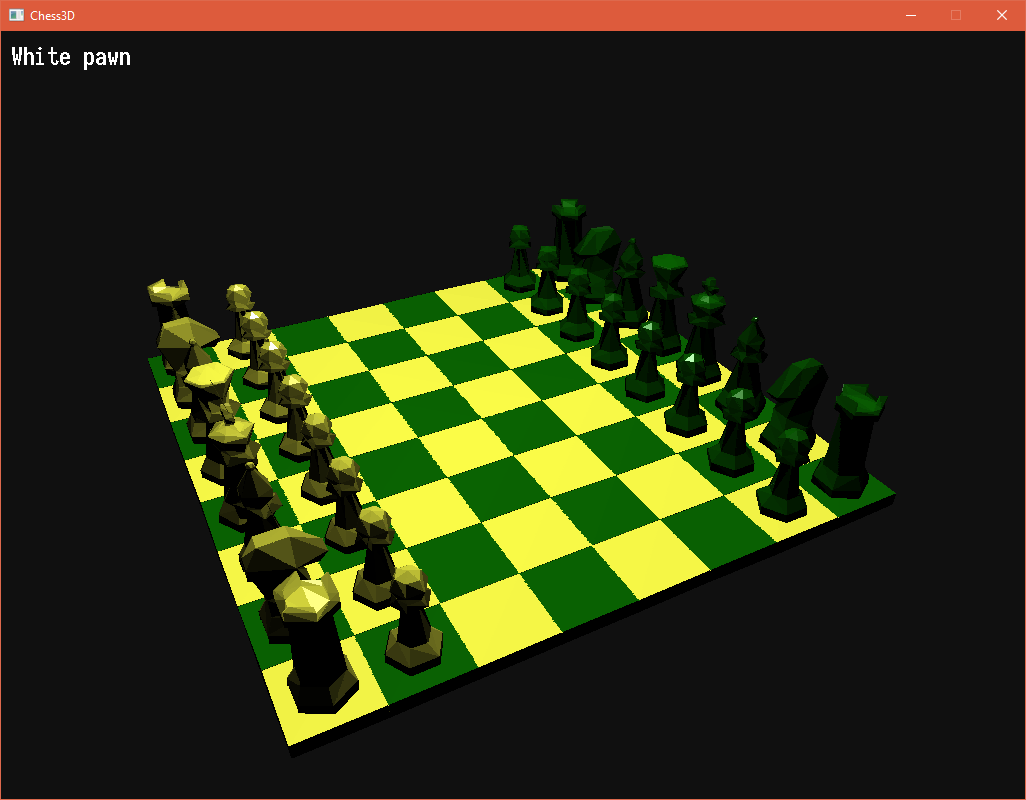
\includegraphics[width=\textwidth]{screenshots/01_pawn_select.png}
		\caption{Wybór pionka}
	\end{subfigure}
	\begin{subfigure}[b]{0.45\textwidth}
		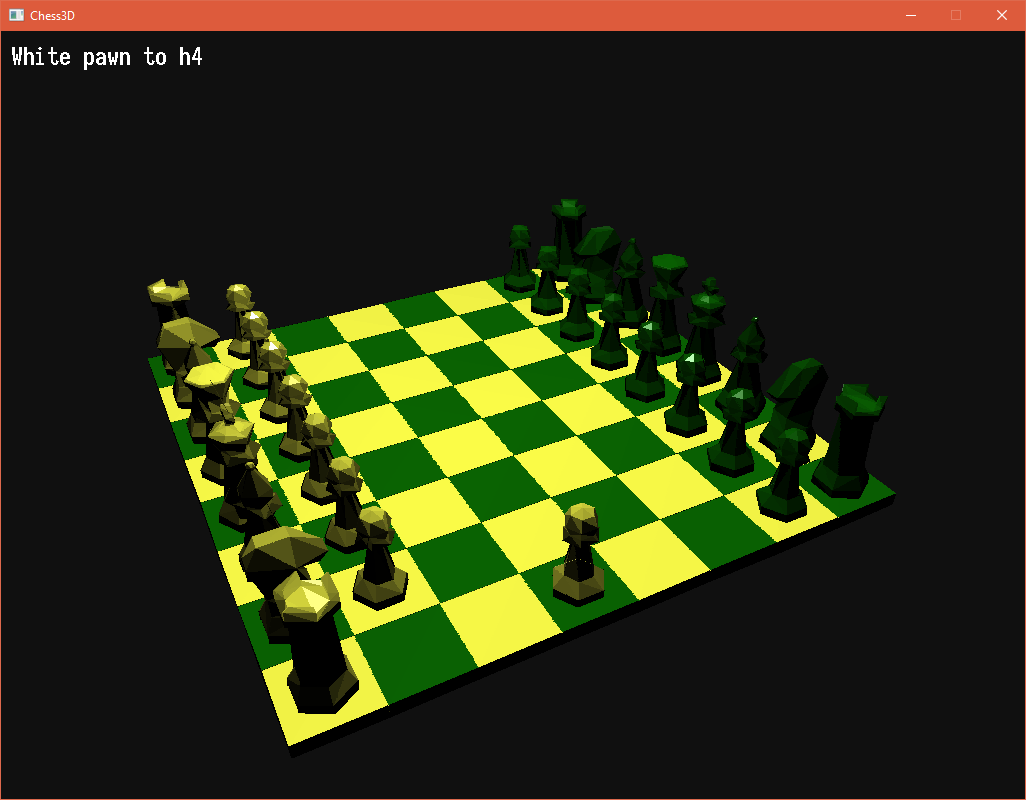
\includegraphics[width=\textwidth]{screenshots/02_move_complete.png}
		\caption{Wykonany ruch}
	\end{subfigure}
	\caption{Wykonanie pojedynczego ruchu przez użytkownika}
\end{figure}

\paragraph{Zmiana kamery}
W dowolnym momencie można dokonać zmiany kamery, wciskając jeden z następujących klawiszy na klawiaturze:
\begin{itemize}
	\item \keystroke{1} -- kamera statyczna, z widokiem na całą planszę,
	\item \keystroke{2} -- kamera o stałym położeniu, śledząca ostatnio poruszony pionek,
	\item \keystroke{3} -- kamera ruchoma, związana z ostatnio poruszonym pionkiem.
\end{itemize} 

\begin{figure}[H]
	\centering
	\begin{subfigure}[b]{0.3\textwidth}
		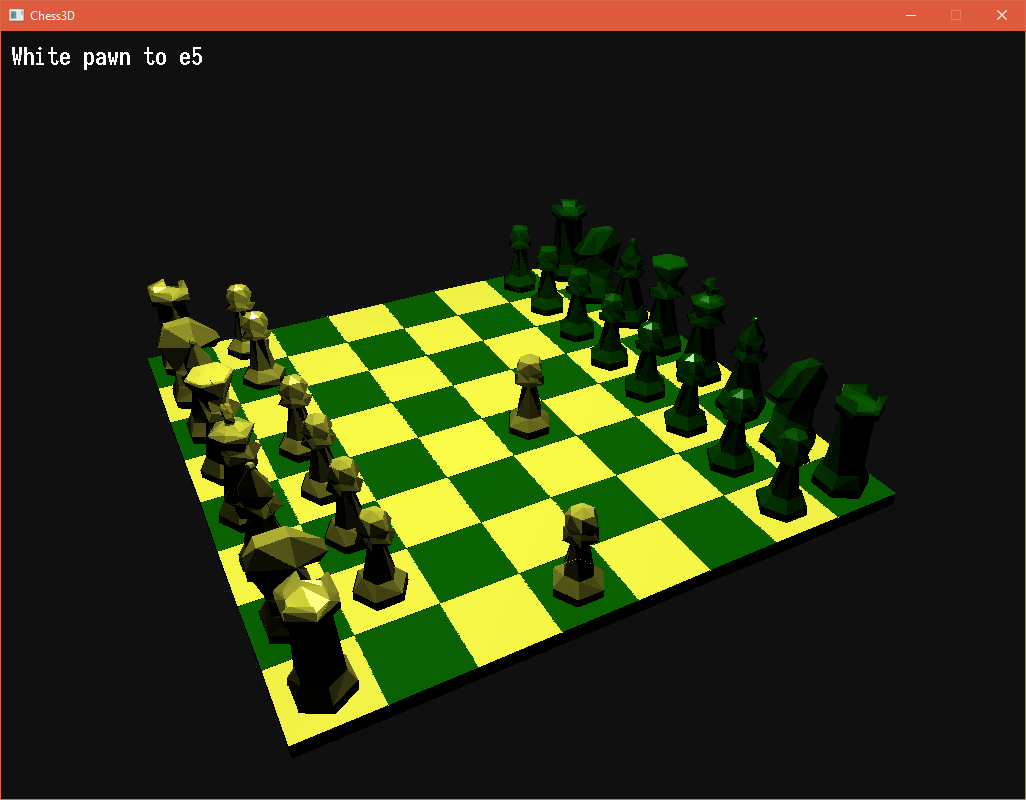
\includegraphics[width=\textwidth]{screenshots/03_static.png}
		\caption{Kamera statyczna (\keystroke{1})}
	\end{subfigure}
	\begin{subfigure}[b]{0.3\textwidth}
		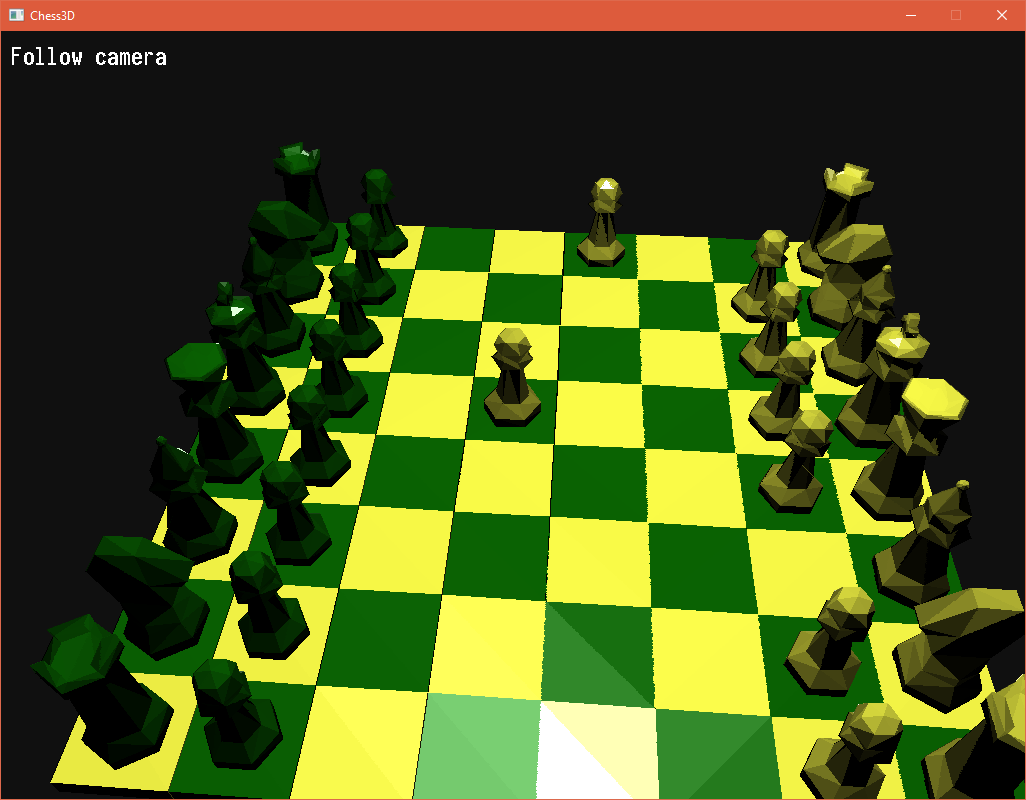
\includegraphics[width=\textwidth]{screenshots/04_follow.png}
		\caption{Kamera śledząca (\keystroke{2})}
	\end{subfigure}
	\begin{subfigure}[b]{0.3\textwidth}
		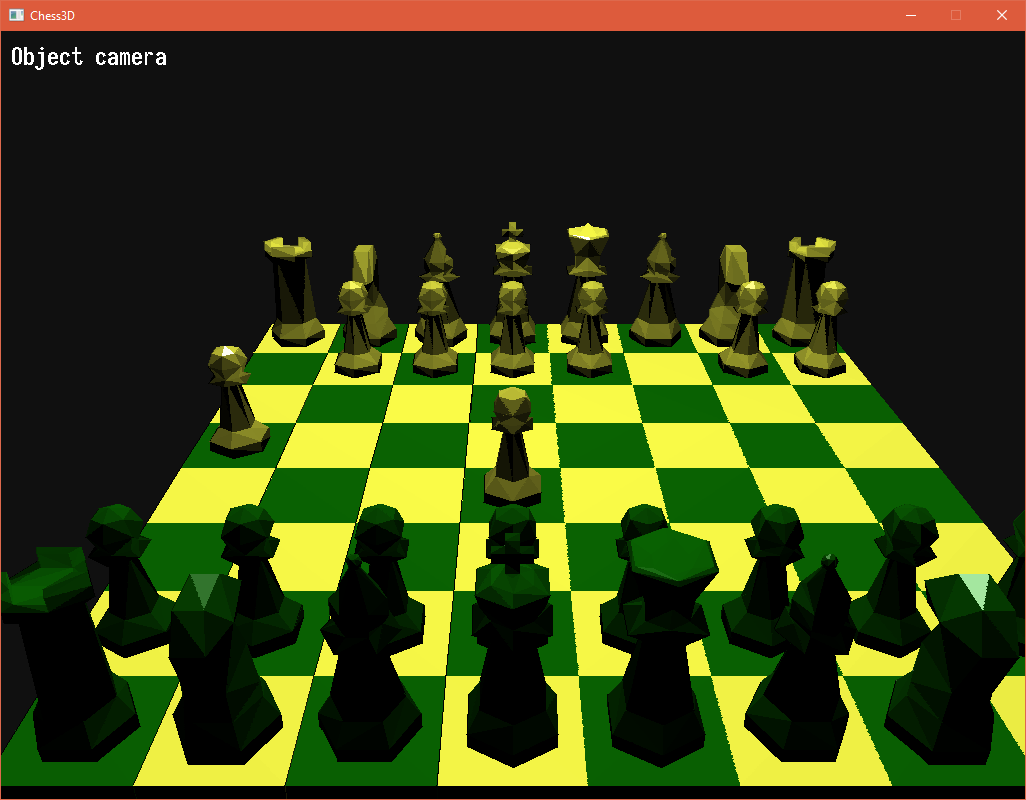
\includegraphics[width=\textwidth]{screenshots/05_object.png}
		\caption{Kamera obiektu (\keystroke{3})}
	\end{subfigure}
	\caption{Dostępne warianty kamery}
\end{figure}

\paragraph{Zmiana modelu oświetlenia}
Podczas działania aplikacji można zmieniać model oświetlenia używany do liczenia kolorów poszczególnych obiektów za pomocą klawiszy:
\begin{itemize}
	\item \keystroke{Q} -- model Blinna-Phonga \cite{blinn77},
	\item \keystroke{W} -- model Phonga \cite{phong75}.
\end{itemize}

\begin{figure}[H]
	\centering
	\begin{subfigure}[b]{0.45\textwidth}
		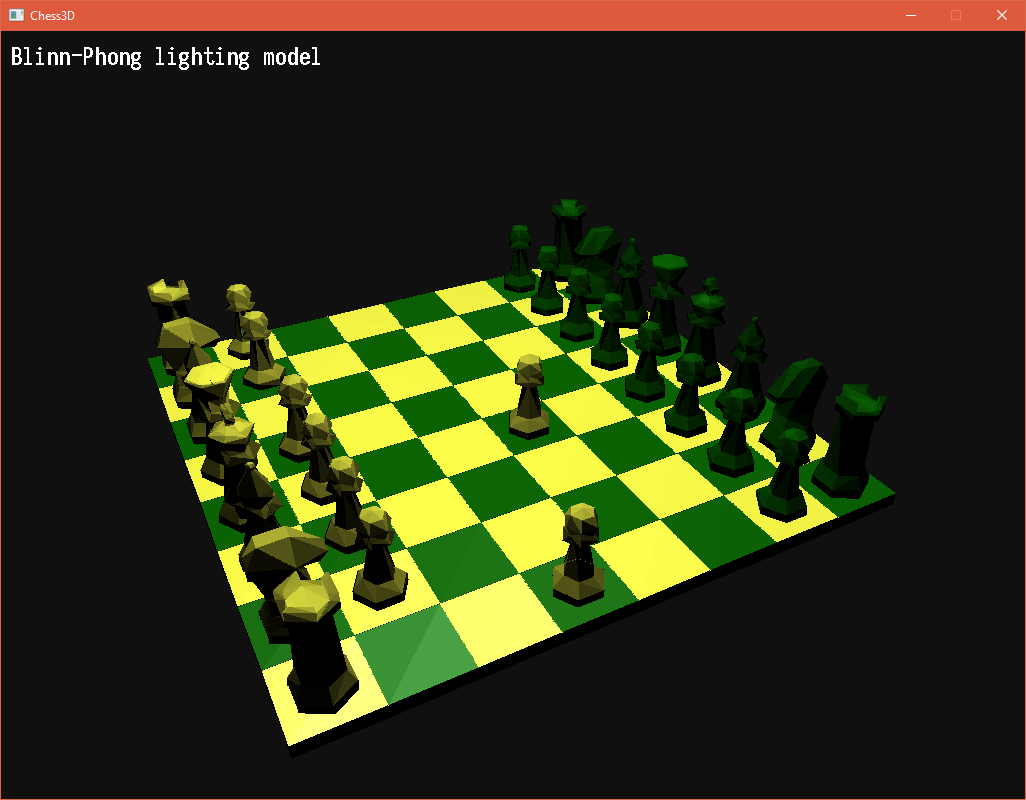
\includegraphics[width=\textwidth]{screenshots/06_blinn-phong.png}
		\caption{Model Blinna-Phonga (\keystroke{Q})}
	\end{subfigure}
	\begin{subfigure}[b]{0.45\textwidth}
		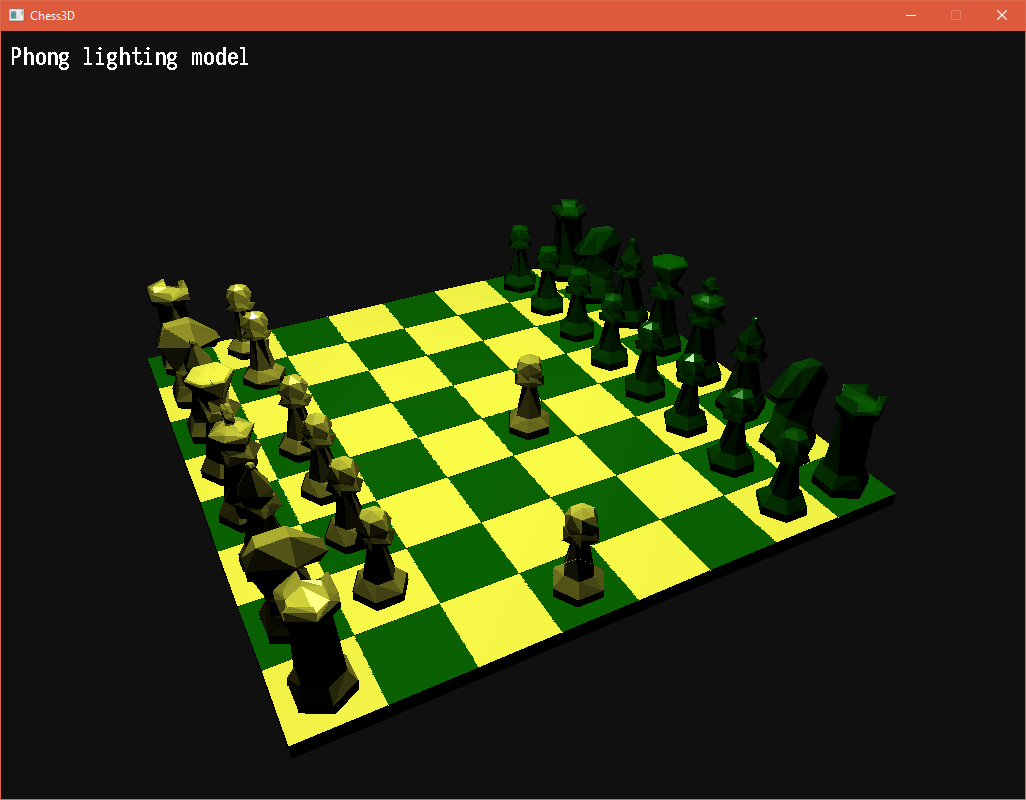
\includegraphics[width=\textwidth]{screenshots/07_phong.png}
		\caption{Model Phonga (\keystroke{W})}
	\end{subfigure}
	\caption{Dostępne modele oświetlenia}
\end{figure}

\paragraph{Zmiana typu cieniowania}
W podobny sposób można modyfikować wykorzystywany w scenie model cieniowania, za pomocą klawiszy:
\begin{itemize}
	\item \keystroke{E} -- cieniowanie płaskie,
	\item \keystroke{R} -- cieniowanie Gouraud \cite{gouraud71},
	\item \keystroke{T} -- cieniowanie Phonga.
\end{itemize}
\subparagraph{Uwaga} Wybrany sposób cieniowania ma znaczący wpływ na prędkość animacji.

\begin{figure}[H]
	\centering
	\begin{subfigure}[b]{0.3\textwidth}
		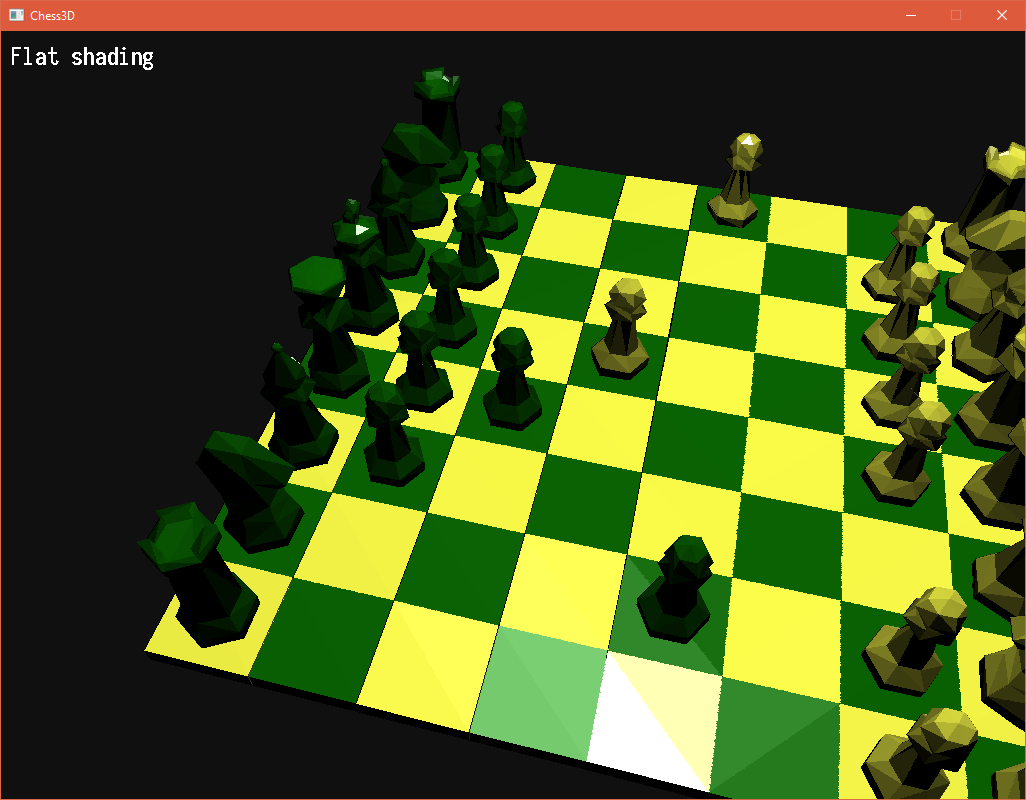
\includegraphics[width=\textwidth]{screenshots/08_flat.png}
		\caption{Cieniowanie płaskie (\keystroke{E})}
	\end{subfigure}
	\begin{subfigure}[b]{0.3\textwidth}
		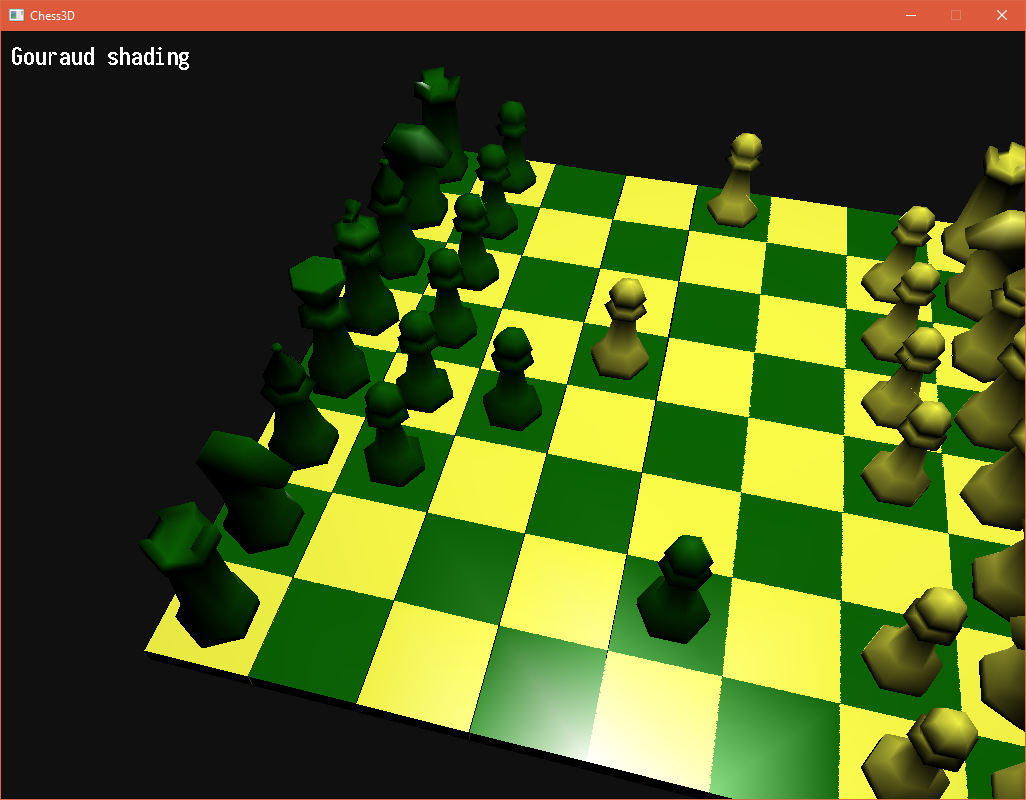
\includegraphics[width=\textwidth]{screenshots/09_gouraud.png}
		\caption{Cieniowanie Gouraud (\keystroke{R})}
	\end{subfigure}
	\begin{subfigure}[b]{0.3\textwidth}
		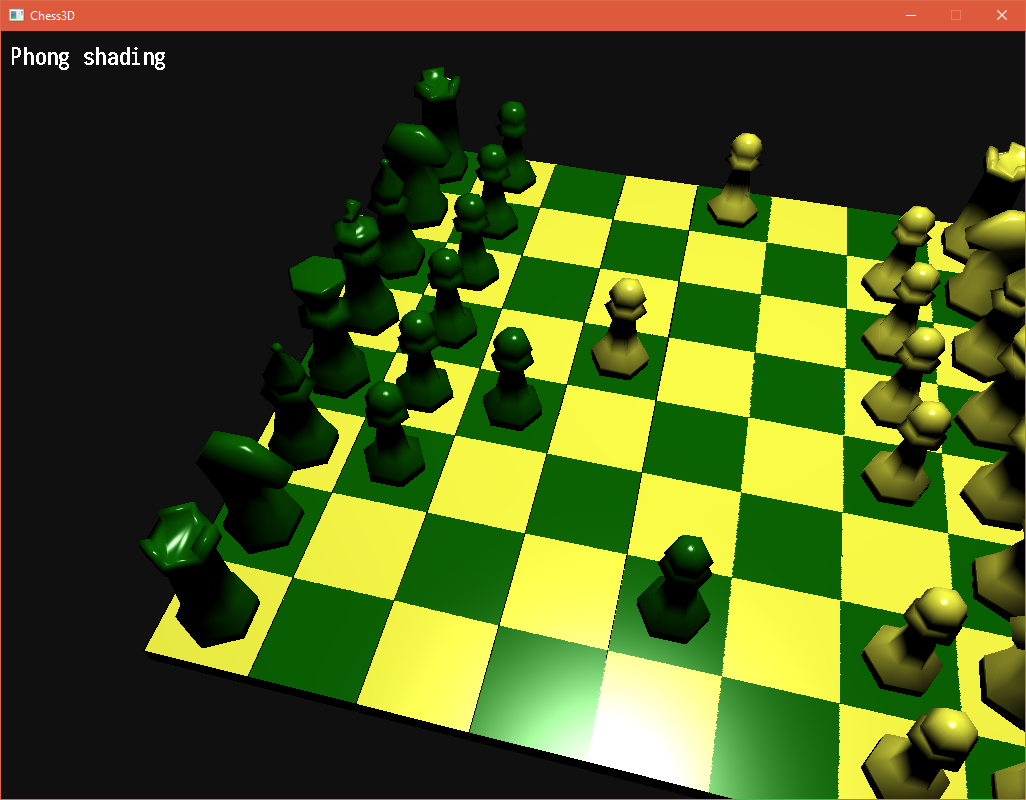
\includegraphics[width=\textwidth]{screenshots/10_phong_shading.png}
		\caption{Cieniowanie Phonga (\keystroke{T})}
	\end{subfigure}
	\caption{Dostępne warianty kamery}
\end{figure}

\subsection{Raport odstępstw od specyfikacji wymagań}

\paragraph{Rezygnacja z implementacji widoku pełnoekranowego}
\subparagraph{Dotyczy:} Wymaganie niefunkcjonalne -- tryby: okienkowy oraz pełnoekranowy
\subparagraph{Zmiana:} Rezygnacja z realizacji wymagania
\subparagraph{Uzasadnienie:} Wymaganie ma stosunkowo niskie znaczenie, a jego realizacja spowodowałaby spadek wydajności aplikacji.

\section{Dokumentacja końcowa (powykonawcza) -- punkty wymagane przez prowadzącego zajęcia}

%\subsection{Pseudokod}

\subsection{Scenariusz i wyniki testów akceptacyjnych}

\begin{tabularx}{\textwidth}{|l|X|}
	\hline
	\textbf{Nazwa testu} & Poruszanie pionkiem \\
	\hline
	\textbf{Opis} & Wybranie dowolnego pionka znajdującego się na planszy przez kliknięcie lewym przyciskiem myszy, a następnie wybranie dowolnego pola planszy. \\
	\hline
	\textbf{Oczekiwany wynik} & Rozpoczęcie się animacji przesuwania się wybranego pionka na wybrane pole. \\
	\hline
	\textbf{Wynik testu} & Pozytywny \\
	\hhline{==}
	\textbf{Nazwa testu} & Zmiana kamery \\
	\hline
	\textbf{Opis} & Wciśnięcie przycisków \keystroke{1}, \keystroke{2}, \keystroke{3} na klawiaturze podczas działania programów. \\
	\hline
	\textbf{Oczekiwany wynik} & Zmiana kamery używanej do wyświetlania sceny. \\
	\hline
	\textbf{Wynik testu} & Pozytywny \\
	\hhline{==}
	\textbf{Nazwa testu} & Zmiana oświetlenia \\
	\hline
	\textbf{Opis} & Wciśnięcie przycisków \keystroke{Q}, \keystroke{W} na klawiaturze podczas działania programów. \\
	\hline
	\textbf{Oczekiwany wynik} & Widoczna zmiana obrazu wyświetlanego na ekranie, oraz wiadomość potwierdzająca zmianę modelu oświetlenia używanego w renderingu sceny. \\
	\hline
	\textbf{Wynik testu} & Pozytywny \\
	\hhline{==}
	\textbf{Nazwa testu} & Zmiana modelu cieniowania \\
	\hline
	\textbf{Opis} & Wciśnięcie przycisków \keystroke{E}, \keystroke{R}, \keystroke{T} na klawiaturze podczas działania programów. \\
	\hline
	\textbf{Oczekiwany wynik} & Widoczna zmiana obrazu wyświetlanego na ekranie, oraz wiadomość potwierdzająca zmianę modelu cieniowania sceny. \\
	\hline
	\textbf{Wynik testu} & Pozytywny \\
	\hhline{==}
	\textbf{Nazwa testu} & Sprawdzenie zużycia pamięci \\
	\hline
	\textbf{Opis} & Uruchomienie programu oraz menedżera zadań, sprawdzenie zużycia pamięci aplikacji. \\
	\hline
	\textbf{Oczekiwany wynik} & Zużycie pamięci RAM przez aplikację nie przekraczające 500 MB. \\
	\hline
	\textbf{Wynik testu} & Pozytywny \\
	\hline
\end{tabularx}

\section{Lista użytych skrótów}

\label{abbr:bsd}
\paragraph{BSD} Berkeley Software Distribution

\label{abbr:mpl}
\paragraph{MPL} Mozilla Public License

\label{abbr:gpu}
\paragraph{GPU} Graphics Processing Unit

\renewcommand*{\refname}{\vspace*{-2em}}
\section{Bibliografia}
\begin{thebibliography}{99}

\bibitem{assimp}
	Assimp -- Open Asset Import Library,
	\url{http://www.assimp.org/}

\bibitem{blinn77}
	James F. Blinn,
	\emph{Models of Light Reflection for Computer Synthesized Pictures},
	Proceedings of the 4th Annual Conference on Computer Graphics and Interactive Techniques,
	pp. 192-198.

\bibitem{eigen}
	Eigen,
	\url{http://eigen.tuxfamily.org/}

\bibitem{freetype}
	FreeType,
	\url{https://www.freetype.org/}
	
\bibitem{gouraud71}
	Henri Gouraud,
	\emph{Continuous Shading of Curved Surfaces},
	IEEE Transactions on Computers,
	June 1971, Volume C-20, Number 6,
	pp. 87-93.

\bibitem{phong75}
	Bui Tuong Phong,
	\emph{Illumination for Computer Generated Pictures},
	Communications of the ACM,
	June 1975, Volume 18, Number 6,
	pp. 311-317.

\bibitem{sdl}
	Simple DirectMedia Layer,
	\url{https://www.libsdl.org/}

\bibitem{sdl_ttf}
	SDL\_ttf 2.0,
	\url{https://www.libsdl.org/projects/SDL_ttf/}
\end{thebibliography}
\end{document}